\chapter{Introduction to Logic}

The word \emph{logic} is used in two senses:
\begin{itemize}
    \item A set of principles that underlie the organization of elements within a system (e.g., a computer program, an electronic device, a communication protocol)
    \item Reasoning conducted according to strict rules that preserve validity
\end{itemize}
In computer science, these two meanings converge: first, we formally describe the given system, and then we \emph{formally reason} about it (in practical applications, this is done automatically), i.e., we derive valid \emph{inferences} about the system using some \emph{(formal) proof system}.

Practical applications of logic in computer science include software verification, logic programming, SAT solving, automated reasoning, database theory, knowledge-based representation, and many others. Moreover, logic (to a greater extent than mathematics) is a fundamental tool for describing theoretical computer science.


\section{Propositional Logic}

Now let's demonstrate logic in action with two real-life examples (from the lives of a treasure hunter and a theoretical computer scientist):


\subsection{Example: Treasure Hunting}

\begin{tcolorbox}
\begin{example}
While searching for treasure in a dragon's lair, we encountered a fork in the path with two corridors. We know that at the end of each corridor, there is either treasure or a dragon, but not both. A dwarf we met at the fork told us, ``At least one of these two corridors leads to the treasure,'' and after some further urging (and a small bribe), she also said, ``The first corridor leads to a dragon.'' It is well known that dwarves you meet in a dragon's lair either always tell the truth or always lie. Which way should we go?
\end{example}
\end{tcolorbox}


\subsection{Formalization in Propositional Logic}

We will begin by formalizing the situation and our knowledge in propositional logic. A \emph{proposition} is a statement to which we can assign a truth value: \emph{True} (1) or \emph{False} (0). Some propositions can be expressed using simpler propositions and logical connectives, e.g., ``(The dwarf is lying) \emph{if and only if} (the second corridor leads to a dragon)'' or ``(The first corridor leads to treasure) \emph{or} (the first corridor leads to a dragon).'' If a proposition cannot be decomposed in this way, it is called a \emph{simple proposition}, \emph{atomic proposition}, or \emph{propositional variable}.

Thus, we will describe the entire situation using \emph{propositional variables}. We can also think of these as simple yes/no questions we need to answer to know everything about the given situation. Let's choose ``The treasure is in the first corridor'' (denote as \(p_1\)), and ``The treasure is in the second corridor'' (\(p_2\)). Other propositional variables could be considered, such as ``There is a dragon in the first corridor'' (\(d_1\)) or ``The dwarf is telling the truth'' (\(t\)). However, these can be expressed using \(\{p_1, p_2\}\), e.g., \(t\) holds if and only if \(p_1\) does not hold. That is, if we know the truth values of \(p_1, p_2\), the truth values of \(d_1, t\) are uniquely determined. A smaller number of propositional variables means a smaller search space.

Next, we will express all our knowledge as (\emph{compound}) propositions and write them in formal notation in the \emph{language} of propositional logic over the set of atomic propositions \( \mathbb{P} = \{p_1, p_2\} \), using symbols representing logical connectives: \( \neg \) (``not X'', \emph{negation}), \( \land \) (``X and Y'', \emph{conjunction}), \( \lor \) (``X or Y'', \emph{disjunction}), \( \limplies \) (``if X, then Y'', \emph{implication}), \( \liff \) (``X if and only if Y'', \emph{equivalence}), and parentheses (, ). It is worth mentioning that disjunction is not exclusive; that is, ``X or Y'' holds even if both X and Y hold, and implication is purely logical: ``if X, then Y'' holds whenever X does not hold or Y holds.

The information that the corridor contains either a treasure or a dragon, but not both, is already encoded in our choice of propositional variables: the presence of a dragon is the same as the absence of treasure. The dwarf's statement that ``The first corridor leads to a dragon'' is thus expressed as ``It is not the case that the treasure is in the first corridor,'' formally \(\neg p_1\). The statement that ``At least one of these two corridors leads to the treasure'' is expressed as ``The treasure is in the first corridor or the treasure is in the second corridor,'' formally \( p_1 \lor p_2\). The information that dwarves either always tell the truth or always lie can be understood to mean that either both our propositions hold or the negations of both our propositions hold, formally:
\[
    (\neg p_1 \land (p_1 \lor p_2)) \lor (\neg (\neg p_1) \land \neg (p_1 \lor p_2))
\]
Let us denote this proposition as \( \varphi \) (from the word ``formula''; propositions are sometimes also called \emph{propositional formulas}). In our example, all information can be expressed with a single proposition. But in practice, we often need more propositions, sometimes even infinitely many (for example, if we want to describe the execution of a computer program and we do not know in advance how many steps it will take). We then describe the situation using a set of propositions, called a \emph{theory}, here \( T = \{ \varphi \} \). The propositions in \( T \) are also called \emph{axioms} of the theory~\( T \)\footnote{Terminology in logic often comes from its application in mathematics.}.


\subsection{Models and Consequences}

Is our information sufficient to determine whether there is treasure in one particular corridor? In other words, we are asking if one of the propositions \( p_1 \) or \( p_2 \) is a logical \emph{consequence} of the proposition \( \varphi \) (or the theory \( T \)). What does this mean?

Let's imagine that there are several ``worlds'' differing in what is at the end of the first and second corridors. For example, in one of the worlds, there is treasure at the end of the first corridor and a dragon at the end of the second corridor. We can describe this world using a truth valuation of the propositional variables: \( p_1 = 1, p_2 = 0 \). Such a valuation is called a \emph{model} of the language \( \mathbb{P} = \{p_1, p_2\} \) and we write it succinctly as \( v = (1,0) \) (\(v\) from the word ``valuation''). Thus, we have a total of four different worlds, described by the \emph{models of the language}:
\[
    \M_\mathbb{P} = \{(0,0), (0,1), (1,0), (1,1)\}.
\]

Is the world described by the model \( v = (1,0) \) consistent with the information we have, i.e., does the proposition \( \varphi \) (or the theory \( T \)) \emph{hold} in it? We can easily determine the truth value of the (compound) proposition \( \varphi \) in the model \(v\), denote it \( v(\varphi) \): We know that \( v(p_1) = 1 \) and \( v(p_2) = 0 \), so \( v(\neg p_1) = 0 \), and also \( v(\neg p_1 \land (p_1 \lor p_2)) = 0 \) (it is a conjunction of two propositions, and the first conjunct is false in the model \( v \)). Similarly, \( v(p_1 \lor p_2) = 1 \) (because \( v(p_1) = 1 \)), so \( v(\neg(p_1 \lor p_2)) = 0 \), and \( v(\neg (\neg p_1) \land \neg (p_1 \lor p_2)) = 0 \). The proposition \( \varphi \) is a disjunction of two propositions, neither of which holds in the model \(v\), so \( v(\varphi) = 0 \).

A keen reader will surely see the tree structure of the proposition \( \varphi \) and the step-by-step evaluation of \( v(\varphi) \) from the leaves to the root. We will present a formal definition in the next chapter.

Similarly, we determine the truth values of the proposition \( \varphi \) in other models. We find that the set of \emph{models of the proposition} \( \varphi \) (or the \emph{models of the theory} \( T \)), i.e., the set of all models of the language in which \( \varphi \) (or all axioms of the theory \( T \)) holds, is
\[
    \M_\mathbb{P}(\varphi) = \M_\mathbb{P}(T) = \{(0,1)\}.
\]
We see that our information uniquely determines the model \( (0,1) \), the world in which there is a dragon in the first corridor and treasure in the second corridor. In general, there can be more models; we only need to know that in every model of \( \varphi \) (or of \(T \)) the proposition \( p_2 \) holds, to conclude that \( p_2 \) is a \emph{consequence} of the theory \( T \); we also say that \( p_2 \) \emph{holds} in the theory \( T \).


\subsection{Proof Systems}

The approach we have chosen is very inefficient. If we have \( n \) propositional variables\footnote{In practice, we commonly have thousands of variables.}, there are \( 2^n \) models of the language, and it is practically impossible to check the validity of the theory in each of them. This is where \emph{proof systems} come into play. In a given proof system, a \emph{proof} of a proposition \( \psi \) from a theory \( T \) is a precisely, formally defined syntactic object that includes an easily (mechanically) verifiable ``proof'' (reason) that \( \psi \) holds in \( T \), and which can be searched for (using a computer) purely based on the structure of the proposition \( \psi \) and the axioms of the theory \( T \) (``syntax''), i.e., without having to deal with models (``semantics'').

We want two properties from a proof system:
\begin{itemize}
    \item \emph{soundness}, i.e., if we have a proof of \( \psi \) from \( T \), then \( \psi \) holds in \( T \), and
    \item \emph{completeness}, i.e., if \( \psi \) holds in \( T \), then there exists a proof of \( \psi \) from \( T \),
\end{itemize}
where soundness is a necessity (without it, searching for proofs makes no sense), and completeness is a desirable property, but an efficient proof system can be useful even if not everything that holds can be proven.

Here we briefly outline two proof systems: the \emph{method of analytic tableaux} and the \emph{resolution method}. They will be formally introduced later, and we will prove soundness and completeness for both of them. Both of these proof systems are based on \emph{proof by contradiction}, i.e., they assume the validity of the axioms from \( T \) and the negation of the proposition \( \psi \), and try to reach a contradiction.


\subsection{Tableau Method}

In the method of analytic tableaux, the `proof' is a \emph{tableau}: a tree whose nodes are labeled with assumptions about the validity of propositions. Let's look at an example of a tableau in Figure~\ref{figure:tableaux-proof-example}.

\begin{figure}
    \centering
    \begin{forest}
    [False \( p_2 \)
        [True \( (\neg p_1 \land (p_1 \lor p_2)) \lor (\neg (\neg p_1) \land \neg (p_1 \lor p_2)) \) 
            [True \( \neg p_1 \land (p_1 \lor p_2) \)
                [True \( \neg p_1 \)
                    [True \( p_1 \lor p_2 \)
                        [False \( p_1 \)
                            [True \( p_1 \), tikz={\node[fit to=tree,label=below:\emph{fail}] {};}
                            ]
                            [True \( p_2 \), tikz={\node[fit to=tree,label=below:\emph{fail}] {};}
                            ]
                        ]
                    ]
                ]
            ]
            [True \( \neg (\neg p_1) \land \neg (p_1 \lor p_2) \)
                [True \( \neg (\neg p_1) \)
                    [True \(\neg (p_1 \lor p_2) \)
                        [False \( (\neg p_1) \)
                            [True \( p_1 \)
                                [False \(p_1 \lor p_2 \)
                                    [False \(p_1\)
                                        [False \(p_2\), tikz={\node[fit to=tree,label=below:\emph{fail}] {};}
                                        ]
                                    ]
                                ]
                            ]
                        ]
                    ]
                ]
            ]
        ]
    ]
    \end{forest}
    \caption{Tableau proof of the proposition \( p_2 \) from the theory \( T \)}\label{figure:tableaux-proof-example}
\end{figure}

We start with the assumption that the proposition \( p_2 \) does not hold (because we are proving by contradiction). Then we add the validity of all axioms of the theory \( T \) (in our case, there is only one: the proposition \( \varphi \) constructed above). We then build the tableau by simplifying the propositions in the assumptions according to certain rules that ensure the following invariant:

\begin{tcolorbox}
\emph{Every model of the theory \( T \) in which \( p_2 \) does not hold must \emph{agree} with one of the branches of the tableau (i.e., satisfy all assumptions on that branch).}
\end{tcolorbox}

The proposition \( \varphi \) is a disjunction of two propositions, \( \varphi = \varphi_1 \lor \varphi_2 \). If it holds in some model, then either \( \varphi_1 \) holds in that model or \( \varphi_2 \) holds in it. We branch the tree according to these two possibilities. In the next step, we have the assumption that the proposition \( \neg p_1 \land (p_1 \lor p_2) \) is true. In that case, both \( \neg p_1 \) and \( p_1 \lor p_2 \) must hold, so we add both of these assumptions to the end of the branch. The truth of \( \neg p_1 \) means the falsity of \( p_1 \), and so on.

We proceed in this manner until it is no longer possible to simplify the propositions in the assumptions, i.e., until they are just propositional variables. If we find a pair of opposite assumptions about some proposition \( \psi \) on one branch, i.e., that it both holds and does not hold, we know that no model can agree with this branch. Such a branch is called \emph{contradictory}. Since we are proving by contradiction, a proof is a tableau in which every branch is contradictory. This ensures that there is no model of \( T \) in which \( p_2 \) does not hold. From this, it follows that \( p_2 \) holds in every model of \( T \), in other words, it is a consequence of \( T \), which is what we wanted to prove.

For now, we will be satisfied with understanding the basic idea of this method; the details will be presented later in Chapter \ref{chapter:tableau-method-propositional}.


\subsection{Resolution Method}

It is not difficult to program a systematic search for a tableau proof. In practice, however, another proof system is used that has a much simpler and more efficient implementation: the \emph{resolution method}. This method dates back to 1965 and forms the basis of most \emph{automated reasoning systems}, \emph{SAT solvers}, or Prolog language interpreters (see Subsection \ref{subsection:resolution-in-prolog}).

The resolution method is based on the fact that every proposition can be equivalently expressed in a special form, called \emph{conjunctive normal form (CNF)}. A \emph{literal} is a propositional variable \( p \) or its negation \( \neg p \) (i.e., literals are propositions that just determine the value of a single propositional variable). A disjunction of several literals, e.g., \( p \lor \neg q \lor \neg r \), is called a \emph{clause}. A proposition is in CNF if it is a conjunction of clauses. For every proposition \( \psi \), there is an \emph{equivalent} proposition \( \psi' \) in CNF. Equivalent means having the same meaning (the same models), which we write as \( \psi \sim \psi' \). Later, we will show two methods of conversion to CNF; for now, let’s look at our example: in the proposition
\[
    (\neg p_1 \land (p_1 \lor p_2)) \lor (\neg (\neg p_1) \land \neg (p_1 \lor p_2))
\]
we first replace \( \neg (\neg p_1) \sim p_1 \) and \( \neg (p_1 \lor p_2) \sim (\neg p_1 \land \neg p_2) \):
\[
    (\neg p_1 \land (p_1 \lor p_2)) \lor (p_1 \land \neg p_1 \land \neg p_2)
\]
and then repeatedly use the \emph{distributivity} of \( \lor \) over \( \land \) (imagine \( \lor \) as multiplication and \( \land \) as addition):
\[
    (\neg p_1 \lor p_1) \land (\neg p_1 \lor \neg p_1) \land (\neg p_1 \lor \neg p_2) \land (p_1 \lor p_2 \lor p_1) \land (p_1 \lor p_2 \lor \neg p_1) \land (p_1 \lor p_2 \lor \neg p_2)
\]
This proposition is already in CNF, but we further simplify it: we omit duplicate literals from clauses, and we realize that if a clause contains a pair of opposite literals \( p, \neg p \), it is a \emph{tautology} (true in every model), and we can remove it. We obtain the CNF proposition
\[
    \neg p_1 \land (\neg p_1 \lor \neg p_2) \land (p_1 \lor p_2)
\]
which is equivalent to the original proposition \( \varphi \).
Since we want to prove \( p_2 \) by contradiction, we add the clause \( \neg p_2 \):
\[
    \neg p_1 \land (\neg p_1 \lor \neg p_2) \land (p_1 \lor p_2) \land \neg p_2
\]
The proposition \( p_2 \) holds in the theory \( T \) if and only if this CNF proposition is \emph{unsatisfiable} (has no model). Propositions in CNF will also be written in \emph{set notation}\footnote{In practical implementation, we could use a list of clauses, where each clause is a list of (unique) literals in some chosen order. Again, imagine thousands of propositional variables and clauses.}:
\[
    \left \{ \{\neg p_1\}, \{\neg p_1, \neg p_2\}, \{p_1, p_2\}, \{\neg p_2\} \right \}
\]
The \emph{resolution rule} states that if we have a pair of clauses, one containing the literal \( p \) and the other the opposite literal \( \neg p \), then their \emph{resolvent}, that is, the clause formed by removing the literal \( p \) from the first clause and \( \neg p \) from the second clause and taking the union of the remaining literals, is a logical consequence of the two clauses. For example, from \( p \lor \neg q \lor \neg r \) and \( \neg p \lor \neg q \lor s \), we can derive the resolvent \( \neg q \lor \neg r \lor s \). \emph{Resolution refutation} of a formula in CNF is then a sequence of clauses ending with the \emph{empty clause \( \square \)} (indicating a contradiction), where each clause is either from the given CNF formula or it is a resolvent of some two preceding clauses. In our case:
\[
    \{\neg p_1\}, \{p_1, p_2\}, \{p_2\}, \{\neg p_2\}, \square
\]
The third clause is the resolvent of the first and second, and the fifth is the resolvent of the third and fourth. The resolution can also be naturally represented using a \emph{resolution tree}, where the leaves are clauses from the given formula, and the inner nodes are resolvents of their children:

\begin{center}
\begin{forest}
for tree={grow=north}
[\( \square \)
    [\( \{\neg p_2\} \)]
    [\( \{p_2\} \)
    [{\( \{p_1, p_2\} \)}]
    [\( \{\neg p_1\} \)]
    ]
]
\end{forest}
\end{center}

If the CNF formula had a model, the model would have to satisfy all of its clauses, and thus gradually all the resolvents in the sequence, and finally the empty clause. But no model can satisfy the empty clause (a disjunction of zero possibilities). We therefore have a proof by contradiction and thus know that we will find the treasure in the second corridor.

The details of the resolution method will be presented in Chapter \ref{chapter:propositional-resolution}.


\subsection{Example: Graph Coloring}\label{subsection:example-graph-coloring}

In the second example, we will get a bit closer to applications. Unlike logical puzzles in the form of word problems, various variants of the graph coloring problem appear in a variety of practical tasks, from scheduling problems to the design of physical and network systems to image processing.

\begin{tcolorbox}
\begin{example}\label{example:graph-coloring-intro}
Find a vertex coloring of the following graph using three colors, i.e., assign to its vertices the colors R, G, B in such a way that no edge is monochromatic.
\begin{center}
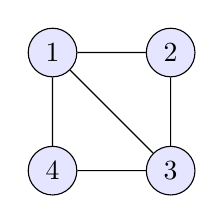
\begin{tikzpicture}[every node/.style={circle,fill=blue!10,draw,minimum size=0.5cm,node distance=1.5cm}]
\node (1) {$1$};
\node[right of=1] (2) {$2$};
\node[below of=2] (3) {$3$};
\node[left of=3] (4) {$4$};
\path[draw] (1) -- (2) -- (3) -- (4) -- (1) -- (3);
\end{tikzpicture}
\end{center}
\end{example}
\end{tcolorbox}

We represent the graph as a set of vertices and a set of edges, where each edge is a pair of vertices. It is easier to work with ordered pairs, so we choose an (arbitrary) orientation of the edges.
\[
\structure G = \langle V; E \rangle = \langle \{1,2,3,4\}; \{(1,2),(1,3),(1,4),(2,3),(3,4)\} \rangle
\]

We start again with formalization in propositional logic. Let the set of colors be \( C = \{R, G, B\} \). The natural choice of propositional variables is ``vertex \( v \) has color \( c \)'', denoted as \( p_v^c \), for each vertex \( v \in V \) and each color \( c \in C \). Our (ordered) set of propositional variables has 12 elements:
\[
\mathbb{P} = \{p_v^c \mid c \in C, v \in V\} = \{p_1^R, p_1^G, p_1^B, p_2^R, p_2^G, p_2^B, p_3^R, p_3^G, p_3^B, p_4^R, p_4^G, p_4^B\}
\]
We have a total of \( |\M_\mathbb{P}| = 2^{12} = 4096 \) models of the language (represented by 12-dimensional 0--1 vectors). Most of them cannot be interpreted as a coloring of the graph. For example, \( v = (1,1,0,0,\dots,0) \) indicates that vertex 1 is colored both red and green. We start with a theory expressing that each vertex has at most one color. There are several ways to express this. We will state, for each vertex, that it must not have (at least) one color from each pair of colors. This gives us a theory in {CNF}:

\begin{align*}
T_1 = \{ 
&(\neg p_1^R \lor \neg p_1^G) \land (\neg p_1^R \lor \neg p_1^B) \land (\neg p_1^G \lor \neg p_1^B),\\
&(\neg p_2^R \lor \neg p_2^G) \land (\neg p_2^R \lor \neg p_2^B) \land (\neg p_2^G \lor \neg p_2^B),\\
&(\neg p_3^R \lor \neg p_3^G) \land (\neg p_3^R \lor \neg p_3^B) \land (\neg p_3^G \lor \neg p_3^B),\\
&(\neg p_4^R \lor \neg p_4^G) \land (\neg p_4^R \lor \neg p_4^B) \land (\neg p_4^G \lor \neg p_4^B)\} \\
    = \{ &(\neg p_v^R \lor \neg p_v^G) \land (\neg p_v^R \lor \neg p_v^B) \land (\neg p_v^G \lor \neg p_v^B) \mid v \in V \} 
\end{align*}
The theory \(T_1\) could be called the theory of \emph{partial} vertex colorings of the graph \(\structure{G}\). The theory \(T_1\) has \(|\M_\mathbb{P}(T_1)| = 4^4 = 2^8 = 256\) models. (Why?) If we want complete colorings, we add the condition that each vertex has at least one color.\footnote{The symbol \(\bigvee \) is used similarly to the symbols \(\sum \) for summation and \(\prod \) for product: to simplify the notation of a proposition in the form of a disjunction. For example, if \(v = 1\), then \( \bigvee_{c \in C} p_v^c \) represents the proposition \( p_1^R \lor p_1^G \lor p_1^B \). Analogously, \(\bigwedge \) for conjunction.}

\begin{align*}
T_2 &= T_1 \cup \{p_1^R \lor p_1^G \lor p_1^B, p_2^R \lor p_2^G \lor p_2^B, p_3^R \lor p_3^G \lor p_3^B, p_4^R \lor p_4^G \lor p_4^B\} \\
    &= T_1 \cup \{ p_v^R \lor p_v^G \lor p_v^B \mid v \in V \} \\
    &= T_1 \cup \{\bigvee_{c \in C} p_v^c \mid v \in V \}  
\end{align*}

The theory \( T_2 \) has \(3^4 = 81\) models. It is an \emph{extension} of the theory \( T_1 \), as every consequence of \( T_1 \) also holds in the theory \( T_2 \). In fact, \( \M_\mathbb{P}(T_2) \subseteq \M_\mathbb{P}(T_1) \).\footnote{Here we see a typical example of the anti-monotonic relationship of the so-called \emph{Galois correspondence}: the more properties (propositions) we require, the fewer objects (models) satisfy these properties.} The remaining condition is to forbid monochromatic edges. For each edge and each color, we specify that at least one of the vertices of the edge must not have the given color. For illustration, we will write out the complete list of propositions one last time; in the future, we will use the abbreviated notation.
\begin{align*}
    T_3 = T_2 \cup \{ & (\neg p_1^R \lor \neg p_2^R) \land (\neg p_1^G \lor \neg p_2^G) \land (\neg p_1^B \lor \neg p_2^B),\\
    & (\neg p_1^R \lor \neg p_3^R) \land (\neg p_1^G \lor \neg p_3^G) \land (\neg p_1^B \lor \neg p_3^B),\\
    & (\neg p_1^R \lor \neg p_4^R) \land (\neg p_1^G \lor \neg p_4^G) \land (\neg p_1^B \lor \neg p_4^B),\\
    & (\neg p_2^R \lor \neg p_3^R) \land (\neg p_2^G \lor \neg p_3^G) \land (\neg p_2^B \lor \neg p_3^B),\\
    & (\neg p_3^R \lor \neg p_4^R) \land (\neg p_3^G \lor \neg p_4^G) \land (\neg p_3^B \lor \neg p_4^B)\} \\  
= T_2 \cup \{ &\bigwedge_{c \in C} 
(\neg p_u^c \lor \neg p_v^c) \mid (u, v) \in E \}
\end{align*}
The resulting theory \( T_3 \) is \emph{satisfiable} (has a model) if and only if the graph \( \structure{G} \) is 3-colorable. It has 6 models. The models are in one-to-one correspondence with 3-colorings of the graph~\( \structure{G} \). The model \( v = (1,0,0,0,1,0,0,0,1,0,1,0) \) corresponds to the following coloring; other colorings can be obtained by permuting the colors.
\begin{center}
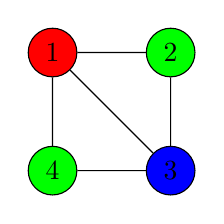
\begin{tikzpicture}[every node/.style={circle,fill=blue!10,draw,minimum size=0.5cm,node distance=1.5cm}]
\node[fill=red] (1) {$1$};
\node[fill=green,right of=1] (2) {$2$};
\node[fill=blue,below of=2] (3) {$3$};
\node[fill=green,left of=3] (4) {$4$};
\path[draw] (1) -- (2) -- (3) -- (4) -- (1) -- (3);
\end{tikzpicture}
\end{center}

Once we have the theory \(T_3\) formalizing 3-coloring of the graph \( \structure{G} \), we can easily solve related questions, such as finding all colorings where vertex 1 is blue and vertex 2 is green: these correspond to the models of the theory \( T_3 \cup \{ p_1^B, p_2^G\} \). Or we can prove that vertices 2 and 4 must be colored the same color. We can use the tableau method: at the root of the tableau will be the assumption
\[
\text{False  }(p_2^R \land p_4^R) \lor (p_2^G \land p_4^G) \lor (p_2^B \land p_4^B)
\]
Or we can find a resolution refutation of the theory formed by converting the axioms of \( T_3 \) into CNF and adding the CNF equivalent of the \emph{negation} of the proposition \( (p_2^R \land p_4^R) \lor (p_2^G \land p_4^G) \lor (p_2^B \land p_4^B) \) (again, because it is a proof by contradiction, we assume for contradiction that the vertices \emph{do not} have the same color).


\section{Predicate Logic}

Now we will very briefly and informally introduce \emph{predicate logic}. Predicate logic deals with properties of objects and relationships between objects. For example:
\begin{quote}\it
    All humans are mortal.\\
    Socrates is a human.\\
    Socrates is mortal.
\end{quote}
In fact, propositional logic emerged later (about a century) than Aristotle's predicate logic, and was largely forgotten for a long time.

\subsection{Disadvantages of Formalization in Propositional Logic}\label{subsection:disadvantages-of-propositional-logic}

The disadvantage of formalizing our graph coloring problem in propositional logic is that the resulting theory \( T_3 \) is quite large and was created ad hoc for the graph \( \structure{G} \). Imagine we need to modify the graph \( \structure{G} \), for example, by adding a new vertex 5 connected by edges to vertices 2 and~3:

\begin{center}
    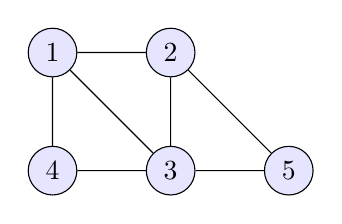
\begin{tikzpicture}[every node/.style={circle,fill=blue!10,draw,minimum size=0.5cm,node distance=1.5cm}]
    \node (1) {$1$};
    \node[right of=1] (2) {$2$};
    \node[below of=2] (3) {$3$};
    \node[left of=3] (4) {$4$};
    \path[draw] (1) -- (2) -- (3) -- (4) -- (1) -- (3);
    \node[right of=3] (5) {$5$};
    \path[draw] (2) -- (5) -- (3);
    \end{tikzpicture}
\end{center}

To formalize the new problem, we need to add three new propositional variables to our language: \(\mathbb{P'} = \mathbb{P} \cup \{ p_5^R, p_5^G, p_5^B \} \), and create new theories \( T'_1, T'_2, T'_3 \) by adding axioms related to vertex 5 and edges \( (2, 5), (3, 5) \). The issue here is that the structure of the graph \( \structure{G} \) and natural properties like ``there is an edge from vertex \( u \) to vertex \( v \)'' or ``vertex \( u \) is green'' have been (`unnaturally') `hardcoded' into 0--1 variables. This drawback is addressed by \emph{predicate logic}.


\subsection{A Brief Introduction to Predicate Logic}

A \emph{model} in predicate logic is not a 0--1 vector but rather a \emph{structure}. Examples of structures are our (oriented) graphs:
\begin{align*}
    &\structure{G} = \langle V^{\structure{G}}; E^{\structure{G}} \rangle = \langle \{1, 2, 3, 4\}; \{(1, 2), (1, 3), (1, 4), (2, 3), (3, 4)\} \rangle \\ 
    &\structure{G}' = \langle V^{\structure{G}'}; E^{\structure{G}'} \rangle = \langle \{1, 2, 3, 4, 5\}; \{(1, 2), (1, 3), (1, 4), (2, 3), (3, 4), (2, 5), (3, 5)\} \rangle
\end{align*}
Both graphs consist of a set of vertices and a binary relation on this set. These are structures in the \emph{language of graph theory} \( \mathcal{L} = \langle E \rangle \), where \(E\) is a binary \emph{relation symbol}. The \emph{language} of predicate logic specifies which relations (how many and of what arity — unary, binary, ternary, etc.) the structures should have, and which symbols we will use for them. Additionally, we use the equality symbol \(=\), and structures can also contain functions and constants (such as the functions \( +, -, \cdot \) and constants \( 0, 1 \) in the \emph{field} of real numbers), but we will leave these for later.

Predicate logic uses the same logical connectives as propositional logic, but the basic building blocks of \emph{predicate formulas} are not propositional variables, but so-called \emph{atomic formulas}, for example: \( E(x, y) \) represents the statement that there is an edge from vertex \( x \) to vertex \( y \) in the graph. Here \( x, y \) are \emph{variables} representing the vertices of the given graph. Additionally, we can use \emph{quantifiers} in the formulas: \( (\forall x) \) ``for all vertices \( x \)'' and \( (\exists y) \) ``there exists a vertex \( y \)''.\footnote{We can think of quantifiers as ``conjunction'' or ``disjunction'' over all vertices of the graph.}

Now we can formalize statements that make sense for any graph. For example: 
\begin{itemize}
    \item ``There are no loops in the graph'': \[ (\forall x)(\neg E(x, x)) \] 
    \item ``There exists a vertex with out-degree 1'': \[ (\exists x)(\exists y)(E(x, y) \land (\forall z)(E(x, z) \limplies y = z)) \] 
\end{itemize}
In the given graph \(\structure{G}\) and under the assignment of vertex \( u \) to the variable \( x \) and vertex \( v \) to the variable \( y \), we evaluate \( E(x, y) \) as True if and only if \( (u, v) \in E^{\structure{G}} \).


\subsection{Formalization of Graph Coloring in Predicate Logic}

Let us return to graph coloring. A natural way to formalize our 3-coloring problem is in the language \( \mathcal{L'} = \langle E, R, G, B \rangle \), where \(E\) is binary and \(R, G, B\) are unary relation symbols, so \(R(x)\) means ``vertex \( x \) is red''. A structure for this language is an (oriented) graph along with a triple of sets of vertices, e.g.,
\begin{align*}
\structure{G}_C &= \langle V^{\structure{G}_C}; E^{\structure{G}_C}, R^{\structure{G}_C}, G^{\structure{G}_C}, B^{\structure{G}_C} \rangle \\
&= \langle \{1, 2, 3, 4\}; \{(1, 2), (1, 3), (1, 4), (2, 3), (3, 4)\}, \{1\}, \{2, 4\}, \{3\} \rangle    
\end{align*}
represents the graph \( \structure{G} \) with the valid coloring from the picture above. We will say that \( \structure{G}_C \) is an \emph{expansion} of the \(\mathcal{L}\)-structure \( \structure{G} \) into the language \( \mathcal{L'} \).

As in propositional logic, we first need to ensure that our models represent colored graphs. We start with the requirement that each vertex is colored with at most one color:
\[
(\forall x)((\neg R(x) \lor \neg G(x)) \land (\neg R(x) \lor \neg B(x)) \land (\neg G(x) \lor \neg B(x)))
\]
We express coloring with at least one color as follows:
\[
(\forall x)(R(x) \lor G(x) \lor B(x))
\]
And we formalize the edge condition using the predicate \( E(x, y) \) as follows:
\[	
(\forall x)(\forall y)(E(x, y) \limplies ((\neg R(x) \lor \neg R(y)) \land (\neg G(x) \lor \neg G(y)) \land (\neg B(x) \lor \neg B(y))))
\]
The models of the resulting theory represent oriented graphs with vertex 3-coloring.


\section{Other Types of Logical Systems}

Predicate logic where variables represent individual vertices is called \emph{first-order} logic (abbreviated as \emph{FO} logic). In \emph{second-order} logic (abbreviated as \emph{SO} logic), we also have variables representing sets of vertices or even sets of \(n\)-tuples of vertices (i.e., relations, functions). For example, the statement that a given graph is bipartite can be formalized in second-order logic with the following formula, where $S$ is a \emph{second-order variable} representing a set of vertices and $S(x)$ expresses that ``vertex $x$ is an element of set $S$'':
$$
(\exists S)(\forall x)(\forall y)(E(x, y) \limplies (S(x) \liff \neg S(y)))
$$
As another important example, consider the statement that every non-empty subset bounded from below has an infimum,\footnote{Which holds in the ordered set of real numbers but not in the rational numbers, e.g., \( \{x \mid x^2 > 2, x > 0\} \).} which can be formalized in second-order logic as follows:\footnote{Even though this formula is quite complex, try to understand its individual parts.}
\begin{align*}
&(\forall S)((\exists x)S(x) \land (\exists x)(\forall y)(S(y) \limplies x \leq y) \limplies {}\\ 
&(\exists x)((\forall y)(S(y) \limplies x \leq y) \land (\forall z)((\forall y)(S(y) \limplies z \leq y) \limplies z \leq x)))
\end{align*}
In \emph{third-order} logic, we even have variables representing sets of sets (which is useful, for example, in topology), etc.

Besides propositional and predicate logic, there are other types of logical systems, such as intuitionistic logic (which only allows constructive proofs), temporal logics (which talk about validity `always', `sometime in the future', `until', etc.), modal logics (`it is possible', `it is necessary'), and fuzzy logic (where we have statements that are `0.35 true'). These logics have important applications in computer science, e.g., in artificial intelligence (modal logics for reasoning of autonomous agents about their environment), in parallel programming (temporal logics), or in washing machines (fuzzy logics). In this course, we will limit ourselves to propositional logic and first-order predicate logic.


\section{About the Lecture}

The lecture is divided into three parts:

The first part deals with propositional logic. First, we introduce syntax and semantics, then the problem of satisfiability of CNF formulas (the well-known NP-complete problem SAT) and its polynomially solvable fragments (2-SAT, Horn-SAT). We will also demonstrate the practical use of a SAT solver. We will continue with the tableau method, proving its soundness and completeness, and several applications, such as the Compactness Theorem. Finally, we will introduce the resolution method in propositional logic.

In the second part, we will introduce predicate logic. Again, we start with syntax and semantics, show how to adapt the tableau method for predicate logic, and end with the resolution method. Additionally, we will mention several practical applications, such as database queries and logic programming (the Prolog language). The structure of the exposition in this part is closely tied to the previous part. Many definitions, theorems, proofs, and algorithms will be very similar to their counterparts in propositional logic. They will mainly differ at the low level, in technical details. Therefore, it is important to have a good understanding of propositional logic before moving on to predicate logic.

The third and smallest part is an introduction to model theory, axiomatizability, and algorithmic decidability. This is a taste of more advanced topics that one  will encounter primarily in theoretical computer science and mathematical logic, although some have their place in applied computer science as well. Finally, we will introduce the famous Gödel's incompleteness theorems, which demonstrate the limits of formal methods (formal provability in an axiomatic system).
